\documentclass[t, aspectratio=169]{beamer}
\usepackage{amsmath,amsfonts,amsthm,amstext,amssymb, xcolor, tikz, pgf, mathrsfs, polynom, pifont, tabto}

% ----------------------------------------------------------
% Theme Setup

% Use Metropolis Theme
\usetheme[numbering=fraction]{metropolis}
\setbeamertemplate{blocks}[rounded][shadow=false]
\makeatletter
\setlength{\metropolis@titleseparator@linewidth}{1pt}
\makeatother

% Define Colors
\definecolor{chargerblue}{HTML}{002764}
\definecolor{chargerred}{HTML}{e02034}
\definecolor{bggray}{HTML}{d0d3d4}

% Set Colors
\setbeamercolor{title}{fg=chargerblue}
\setbeamercolor{background canvas}{bg=white}
\setbeamercolor{title separator}{fg=chargerred}
\setbeamercolor{structure}{fg=chargerblue}
\setbeamercolor{frametitle}{fg=white, bg=chargerblue}
\setbeamercolor*{normal text}{fg=chargerblue}
\setbeamercolor*{block body}{bg=bggray}
\setbeamercolor*{block title}{bg=chargerblue, fg=white}
% ----------------------------------------------------------

% ----------------------------------------------------------
% Custom Definitions, Commands, Environments, etc.

% Sets of numbers
\def\R{\mathbb{R}} % The reals
\def\N{\mathbb{N}} % The naturals
\def\Z{\mathbb{Z}} % The integers
\def\Q{\mathbb{Q}} % The rationals

% Blank space
\newcommand{\blank}[1]{\underline{\hspace{#1}}} % Blank space

% Change font colors
\newcommand{\cyan}[1]{{\color{cyan}{#1}}} % Changes font to cyan
\newcommand{\red}[1]{{\color{red}{#1}}} % Changes font to red
\newcommand{\magenta}[1]{{\color{magenta}{#1}}} % Changes font to magenta
\newcommand{\orange}[1]{{\color{orange}{#1}}} % Changes font to orange
\newcommand{\yellow}[1]{{\color{yellow}{#1}}} % Changes font to yellow
\newcommand{\violet}[1]{{\color{violet}{#1}}} % Changes font to violet
\newcommand{\green}[1]{{\color{green}{#1}}} % Changes font to green
\newcommand{\blue}[1]{{\color{blue}{#1}}} % Changes font to blue
\newcommand{\white}[1]{{\color{white}{#1}}} % Changes font to white

% Fitted inclusion symbols
\newcommand{\fp}[1]{\left({#1}\right)} % Fitted parentheses around content
\newcommand{\fb}[1]{\left[{#1}\right]} % Fitted brackets
\newcommand{\lhoi}[1]{\left({#1}\right]} % Left half-open interval
\newcommand{\rhoi}[1]{\left[{#1}\right)} % Right half-open interval
\newcommand{\set}[1]{\left\{{#1}\right\}} % Fitted braces (useful for sets)
\newcommand{\av}[1]{\left|{#1}\right|} % Fitted absolute value bars

% Augmented Matrix Environment
\newenvironment{amatrix}[1]{%
	\left[\begin{array}{@{}*{#1}{c}|c@{}}
	}{%
	\end{array}\right]
}

% Miscellaneous
\def\then{\Rightarrow}
\def\to{\rightarrow}
\def\d{^{\circ}}
\newcommand{\?}{\stackrel{?}{=}}
\newcommand{\cmark}{\text{ \ding{51}}}
\newcommand{\xmark}{\text{ \ding{55}}}

% Coordinate Plane (Four-Quadrant)
\def\coordplane {
	\begin{tikzpicture}        \draw[step=0.25cm,black,very thin,opacity=0.25] (-2.5cm, -2.5cm) grid (2.5cm, 2.5cm);
		\draw[<->,thick,black] (-2.5cm, 0) -- (2.5cm, 0) node[anchor=north west,pos=0.94,font=\scriptsize]{$x$};
		\draw[<->,thick,black] (0,-2.5cm) -- (0, 2.5cm) node[anchor=south east,font=\scriptsize,pos=0.94]{$y$};
	\end{tikzpicture}
}

% Coordinate Plane (One-Quadrant)
\def\onequad {
	\begin{tikzpicture}
		\draw[step=0.25cm, black, very thin, opacity=0.25] (0,0) grid (7.5cm,5cm);
		\draw[->, thick, black] (0,0) -- (7.5cm, 0) node[anchor=north west,font=\scriptsize,pos=0.94]{$x$};
		\draw[->, black, thick] (0,0) -- (0,5cm) node[anchor=south east,font=\scriptsize,pos=0.94]{$y$};
	\end{tikzpicture}
}
% ----------------------------------------------------------

% ----------------------------------------------------------
% Presentation Information
\title[6-2]{Applications of Normal Distributions}
\subtitle{Section 6-2}
\author{Jacob Ayers}
\institute{Lesson \#18}
\date{MAT 110}
% ----------------------------------------------------------

\begin{document}
	
	% Slide 1 (Title Slide)
	\begin{frame}
		\titlepage
	\end{frame}
	
	% Slide 2 (Objectives)
	\begin{frame}{Objectives}
		\begin{itemize}
			\item Use a graphing calculator to find areas/probabilities under normal distributions
			\item Solve applied problems involving normal distributions
		\end{itemize}
	\end{frame}

	\begin{frame}{Graphing Calculators and Normal Distributions}
		Last lesson, we used a table of values to help us find probabilities and areas under the standard normal distribution. \pause
		
		A graphing calculator can also perform these calculations. \pause
		
		As usual, I'll use the TI-84 Plus to demonstrate, but I'll post a video for Casio users.
	\end{frame}

	\begin{frame}{Graphing Calculators and Normal Distributions}
		Example: Find the area under the standard normal distribution to the right of $z = -0.85$. \pause \\ $0.8023$ \pause
		
		Example: Find the area under the standard normal distribution to the left of $z = -2.01$. \pause \\ $0.0222$ \pause
		
		Example: Find the area under the standard normal distribution between $z = -1.42$ and $z = 1.42$. \pause \\ $0.8444$ \pause
		
		Example: Find $P(0 < z < 3.00)$. \pause \\ $0.4987$
	\end{frame}

	\begin{frame}{Applications of Normal Distributions}
		Many real-world phenomena are normally distributed. \pause
		
		Examples: \begin{itemize}
			\item SAT Scores
			\item Weights of newborns
			\item IQ
		\end{itemize} \pause
	
		These variables do not follow the standard normal distribution; generally $\mu \neq 0$ and $\sigma \neq 1$. \pause
		
		However, we can compute $z$-scores and use those along with the table we saw in the last lesson (or a calculator) to solve them. 
	\end{frame}

	\begin{frame}{Applications of Normal Distributions}
		To solve applied normal distribution problems by hand, follow the procedure below.
		
		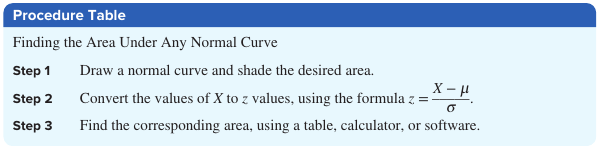
\includegraphics[width=\textwidth]{norm-app-proc.png} \pause
		
		To solve them using a calculator is just a matter of setting your values correctly. \pause
		
		In either case, round to four decimal places.
	\end{frame}

	\begin{frame}{Applications of Normal Distributions}
		An adult has on average 5.2 liters of blood. Assume the variable is normally distributed and has a standard deviation of 0.3. Find the percentage of people who have more than 4.8 liters of blood in their system. \pause
		
		First, draw a picture: \vspace{1 in} \pause
		
		Next, convert the $z$-score: $z = \dfrac{4.8 - 5.2}{0.3} \approx -1.33$ \\ \pause
		Using the table: $P(\text{less than 4.8}) = 0.0918$. \pause So about 9.18\% of people have less than 4.8 liters of blood in their systems.
	\end{frame}

	\begin{frame}{Applications of Normal Distributions}
		Each month, an American household generates an average of 28 pounds of newspaper for garbage or recycling. Assume the variable is approximately normally distributed and the standard deviation is 2 pounds. If a household is selected at random, find the probability of its generating between 27 and 31 pounds of newspaper per month. \pause
		
		First, draw a picture: \vspace{1in} \pause
		
		Next, convert to $z$-scores: $z_1 = \dfrac{27 - 28}{2} = -0.50$ \pause and $z_2 = \dfrac{31 - 28}{2} = 1.50$. \pause \\
		Using the table: $P(27 < X < 31) = 0.9332 - 0.3085 = 0.6247$ (62.47\%)
	\end{frame}

	\begin{frame}{Applications of Normal Distributions}
		The average number of calories in a 1.5-ounce chocolate bar is 225. Suppose that the distribution of calories is approximately normal with $\sigma = 10$. Find the probability that a randomly selected chocolate bar will have more than $208$ calories. \pause
		
		First, draw a picture: \vspace{1in} \pause
		
		Next, convert to a $z$-score: $z = \dfrac{208 - 225}{10} = -1.70$. \\ \pause
		Using the table: $P(X > 208) = 1 - 0.0446 = 0.9554$.
	\end{frame}

	\begin{frame}{Applications of Normal Distributions}
		Another common problem we are interested in solving is finding a ``cutoff score." \pause
		
		Example: The top 20\% of SAT scores earn scholarships - what score do you need to earn? \pause
		
		Again, we can solve these problems by hand or using a calculator. \pause
		
		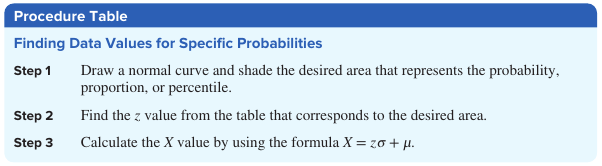
\includegraphics[width=4in]{norm-cutoff-proc.png} \pause
		
		On a calculator, we can use the $invNorm$ command.
	\end{frame}

	\begin{frame}{Applications of Normal Distributions}
		To qualify for a police academy, candidates must score in the top 10\% on a general abilities test. Assume the test scores are normally distributed with a mean of $200$ and standard deviation of $20$. Find the lowest possible score to qualify. \pause
		
		First, draw a picture. \vspace{1in} \pause
		
		Next, compute the probability to the \textit{left}: $1 - 0.1000 = 0.9000$. \pause \\
		Search for $0.9000$ in the table. \pause $z$-score = $1.28$. \pause \\
		So the cutoff is $X = 200 + 1.28\cdot 20 = 225.6 \uparrow 226$
	\end{frame}

	\begin{frame}{Applications of Normal Distributions}
		For a medical study, a researcher wishes to select people in the middle 60\% of the population based on blood pressure. Assuming that blood pressure readings are normally distributed with $\mu = 120$ and $\sigma = 8$, find the upper and lower readings that would qualify people to participate in the study. \pause
		
		First, draw a picture. \pause \vspace{1in}
		
		Now, we need to find an upper cutoff and a lower cutoff. \pause \\
		At the upper cutoff, 80\% of values will be to the left (lookup: $0.8000$). \pause \\
		At the lower cutoff, 20\% of values will be to the left (lookup: $0.2000$).
	\end{frame}

	\begin{frame}{Applications of Normal Distributions}
		Upper cutoff: $z$-score for $0.8000$ is $0.84$; $X = 120 + 0.84(8) = 126.72 \uparrow 127$ \pause
		
		Lower cutoff: $z$-score for $0.2000$ is $-0.84$; $X = 120 - 0.84(8) = 113.28 \downarrow 113$ \pause
		
		Important: Rounding rules are not based on place value. \pause
		
		For upper limits, always round up (because if you round down, your rounded value is below the cutoff). \pause
		
		For lower limits, always round down (because if you round up, your rounded value is above the cutoff).
	\end{frame}

	\begin{frame}{Applications of Normal Distributions}
		A contractor decided to build homes that will include the middle 80\% of the market. If the average size of homes built is 1810 square feet, find the maximum and minimum sizes of homes the contractor should build. Assume that the standard deviation is 90 square feet and the variable is normally distributed. \pause
		
		First, draw a picture. \pause \vspace{1in}
		
		Lookups: \\ \pause
		Upper: $0.9000$ \\ \pause
		Lower: $0.1000$
	\end{frame}

	\begin{frame}{Applications of Normal Distributions}
		Upper Cutoff: $z = 1.28$ so $X = 1810 + 1.28(90) = 1925.2 \uparrow 1926$ \\ \pause
		Lower Cutoff: $z = -1.28$ so $X = 1810 - 1.28(90) = 1694.8 \downarrow 1694$.
	\end{frame}

	\begin{frame}{Next Steps}
		\begin{itemize}
			\item Read 6-3
			\item Watch Video Lesson \#19
			\item Complete Assignment \#9
		\end{itemize}
	
		\vfill
		
		Thanks for watching!
	\end{frame}
	
\end{document}